\documentclass{article}

\usepackage[utf8]{inputenc}
\usepackage[top=1.5in,left=.9in,right=.9in,bottom=1in,headheight=1in]{geometry}
\usepackage{fancyhdr}
\usepackage{lastpage}
\usepackage{amsmath,amssymb,amsthm}
\usepackage{mathrsfs}
\usepackage{multicol}
\usepackage{enumerate}

\usepackage{tkz-graph}
\usetikzlibrary{arrows}



% Better looking empty set
\let\emptyset\varnothing

\newtheoremstyle{problem}{\topsep}{\topsep}%
{}%         Body font
{}%         Indent amount (empty = no indent, \parindent = para indent)
{\bfseries}% Thm head font
{\vspace{5pt}}%        Punctuation after thm head
{\newline}%     Space after thm head (\newline = linebreak)
{\thmname{#1}\thmnote{ #3}}%         Thm head spec

\theoremstyle{problem}
\newtheorem{prob}{Problem}

\theoremstyle{plain}
%\newtheorem{thm}{Theorem}
\newtheorem{lem}{Lemma}
\newtheorem{prop}{Proposition}
% No indent for whole page
\setlength\parindent{0pt}

\theoremstyle{remark}
\newtheorem{countex}{Counterexample}

\setlength{\columnsep}{1cm}
%%% Heading -- No need to edit %%%
\pagestyle{fancy}

\rhead{
  Stefan Eng\\
  Dr. Katherine Stevenson\\
  Math 320\\
  10/16/13
}
\lhead{
  Ch 4: \# 10, 11, 13, 19, 20, 25, 34
}

\cfoot{Page\ \thepage\ of\ \pageref{LastPage}}
%%%

\renewcommand{\qedsymbol}{$\blacksquare$}
% For manual qed box
\def\bs{\hspace{\stretch1}\ensuremath\blacksquare}

\begin{document}

%%% Make the title %%%
\begin{center}
\textsc{\Large Foundations of Higher Mathematics}\\[.3cm]
\textsc{\Large Homework 7}
\end{center}
%%% End title %%%

%%% Start Assignment Here %%%
\begin{prob}[10]

\end{prob}
%

\begin{prob}[11]
\begin{enumerate}[a)]
\item \begin{proof}
Suppose $S \subseteq T$ and $x$ is in the domain of $S$. Then for an arbitrary element $y \in S[x]$, $(x,y) \in S$. Since $S \subseteq T$ and $(x,y) \in S$, then $(x,y) \in T$ and $y \in T[x]$. Therefore, $S[x] \subseteq T[x]$.
\end{proof}
\item \begin{proof}
$(A \times B)[x] = B$ if $x \in A$.
\end{proof}
\end{enumerate}
\end{prob}
%

\begin{prob}[13]

\end{prob}
%

\begin{prob}[19]

\end{prob}
%

\begin{multicols}{2}
\begin{prob}[20a]
  $R = \{(a,b) \in A \times A:a\text{ divides } b\}$\\[5pt]

  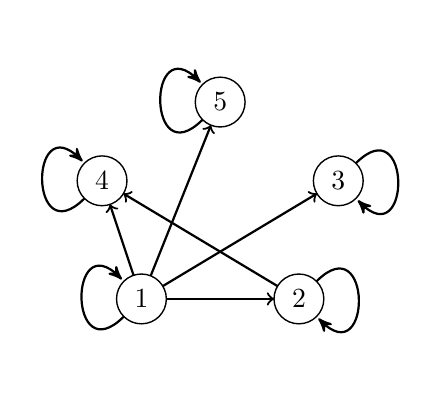
\begin{tikzpicture}
    % Vertices
    \Vertex[x=-1, y=0]{1}
    \Vertex[x=1, y=0]{2}
    \Vertex[x=1.5, y=1.5]{3}
    \Vertex[x=-1.5, y=1.5]{4}
    \Vertex[x=0, y=2.5]{5}

    % Edges
    \tikzset{EdgeStyle/.append style = {-> }}
    % 1 | everything
    \Edge(1)(2) 
    \Edge(1)(3) 
    \Edge(1)(4) 
    \Edge(1)(5) 
    

    % 2 | 4 
    \Edge(2)(4)

    % 3 | 


    % Loops
    \Loop[dist=1cm](1)
    \Loop[dist=1cm,dir=EA](2)
    \Loop[dist=1cm,dir=EA](3)
    \Loop[dist=1cm](4)
    \Loop[dist=1cm](5)

  \end{tikzpicture}
\end{prob}

\begin{prob}[20b]
  $U = \{(a,b) \in A \times A:a \not = b\}$\\[5pt]
  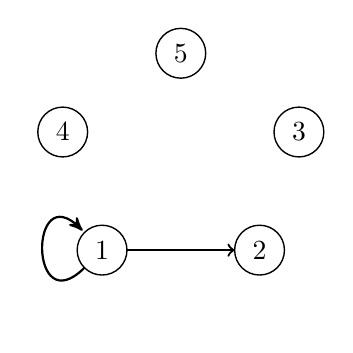
\begin{tikzpicture}
    % Vertices
    \Vertex[x=-1, y=0]{1}
    \Vertex[x=1, y=0]{2}
    \Vertex[x=1.5, y=1.5]{3}
    \Vertex[x=-1.5, y=1.5]{4}
    \Vertex[x=0, y=2.5]{5}

    % Edges
    \tikzset{EdgeStyle/.append style = {-> }}    
    \Edge(1)(2) 
 

    % Loops
    \Loop[dist=1cm](1)
  \end{tikzpicture}
\end{prob}
\vfill
\columnbreak

\begin{prob}[20c]
  $E = \{(a,b) \in A \times B:a + b \text{ is even}\}$\\[5pt]
  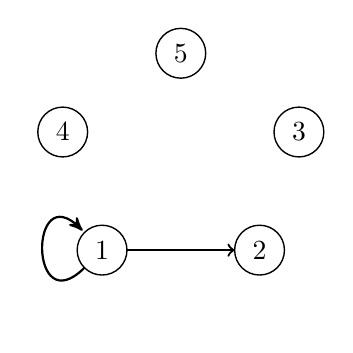
\begin{tikzpicture}
    % Vertices
    \Vertex[x=-1, y=0]{1}
    \Vertex[x=1, y=0]{2}
    \Vertex[x=1.5, y=1.5]{3}
    \Vertex[x=-1.5, y=1.5]{4}
    \Vertex[x=0, y=2.5]{5}

    % Edges
    \tikzset{EdgeStyle/.append style = {-> }}
    \Edge(1)(2) 

    % Loops
    \Loop[dist=1cm](1)
  \end{tikzpicture}
\end{prob}

\begin{prob}[20d]
  $O = \{(a,b) \in A \times B:a + b \text{ is odd}\}$\\[5pt]
  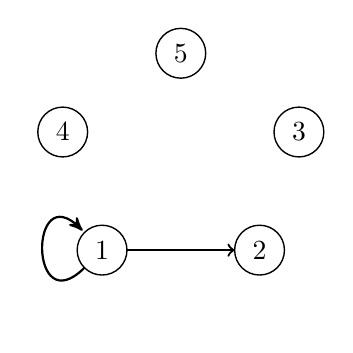
\begin{tikzpicture}
    % Vertices
    \Vertex[x=-1, y=0]{1}
    \Vertex[x=1, y=0]{2}
    \Vertex[x=1.5, y=1.5]{3}
    \Vertex[x=-1.5, y=1.5]{4}
    \Vertex[x=0, y=2.5]{5}

    % Edges
    \tikzset{EdgeStyle/.append style = {-> }}
    \Edge(1)(2) 

    % Loops
    \Loop[dist=1cm](1)
  \end{tikzpicture}
\end{prob}
% 
\end{multicols}


\begin{prob}[25]

\end{prob}
%

\begin{prob}[34]

\end{prob}
%

\end{document}